\documentclass[12pt]{extarticle}
\usepackage[utf8]{inputenc}
\usepackage[left=1.5cm,top=1.5cm,right=1.5cm,bottom=1.5cm]{geometry}
\usepackage{amsmath}
\usepackage{amssymb}
\usepackage{amsfonts}
\usepackage{amstext}
\usepackage{amsthm}
\usepackage{etoolbox}
\usepackage{graphicx}
\usepackage[dvipsnames,table,xcdraw]{xcolor}
\usepackage{mathrsfs}
\usepackage{verbatim} 
\usepackage{multicol}
\usepackage{float}
\usepackage{setspace}
\usepackage{upgreek}
\usepackage{mathtools}
\usepackage{relsize}
\usepackage{cancel}
\usepackage{textgreek}
\usepackage{yfonts}
\usepackage{bbold}
\usepackage{ragged2e}
\usepackage{txfonts}
\usepackage{fancyhdr}

\usepackage{url}
\usepackage{multirow} % Multiple rows in tables
\usepackage{enumitem} % Extra configuration of enums
\usepackage{icomma} % Remove space from decimal comma
\usepackage{hyperref} % For specifying document metadata
\usepackage{array} % For making better matrices
\usepackage[spanish]{babel} % For printing date in spanish
\usepackage[version=4]{mhchem} % For writing chemical formulae

\hypersetup{
    pdftitle={Resumen de Matemática},
    pdfauthor={Ezequiel Mundani Vegega}
}

\linespread{1}

\pagestyle{fancy}
\setlength{\headheight}{15pt}
\lhead{Resumen hecho por Ezequiel Mundani}
\rhead{Para clases particulares: +54 911 4095 5806}

\renewcommand*\contentsname{Índice:}

\setlist[enumerate,1]{label=\arabic*), topsep = 0pt}
\setlist[enumerate,2]{label=\alph*., topsep = 0pt}
\setlist[enumerate]{itemindent=1em, labelsep=1.5em}
\makeatletter
\newcommand*\bigcdot{\mathpalette\bigcdot@{.5}}
\newcommand*\bigcdot@[2]{\mathbin{\vcenter{\hbox{\scalebox{#2}{$\m@th#1\bullet$}}}}}
\makeatother
\newcommand{\skipline}{\vspace{\baselineskip}}
\newcommand{\sskip}{\vspace{0.2cm}} %small skip
\newcommand{\tab}{\hspace{8mm}}

\newcommand{\R}{\mathbb{R}}
\newcommand{\knn}{\mathbb{K}^{n \times n}}
\newcommand{\kn}{\mathbb{K}^{n}}
\newcommand{\rnn}{\mathbb{R}^{n \times n}}
\newcommand{\rmn}{\mathbb{R}^{m \times n}}
\newcommand{\rn}{\mathbb{R}^{n}}
\newcommand{\cnn}{\mathbb{C}^{n \times n}}
\newcommand{\cmn}{\mathbb{C}^{m \times n}}
\newcommand{\cn}{\mathbb{C}^{n}}
\newcommand{\A}{\textgoth{A}}

\newcommand{\ber}{\mathbb{1}}

\newcommand{\fl}{\hspace*{\fill}\\}

\definecolor{lgray}{RGB}{230, 230, 230}
\definecolor{ProbaYellow}{RGB}{0, 75, 100}

\hypersetup{
    pdftitle={Ejercicios de Química},
    pdfauthor={Ezequiel Mundani Vegega}
}

\begin{document}
    \tableofcontents
    \vfill
    \section*{Última actualización: \today}
    \vfill
    \section{Estructura de la materia}

\begin{enumerate}
\item Obtener la cantidad de protones de los átomos de los siguientes elementos:
\begin{multicols}{4}
\begin{enumerate}
    \item Oxígeno
    \item Sodio
    \item Helio
    \item Hierro
    \item Oro
    \item Uranio
    \item Calcio
    \item Yodo
\end{enumerate}
\end{multicols}


\item Obtener la cantidad de protones y electrones de los siguientes átomos:
\begin{multicols}{4}
\begin{enumerate}
    \item \ce{Cl}
    \item \ce{Br^-}
    \item \ce{Mg^{2+}}
    \item \ce{S^{2-}}
    \item \ce{H^{+}}
    \item \ce{Co}
    \item \ce{Fe^{3+}}
    \item \ce{K^{+}}
\end{enumerate}    
\end{multicols}


\item Obtener la cantidad de protones, neutrones, electrones, Z y A de los siguientes átomos:
\begin{multicols}{4}
\begin{enumerate}
    \item \ce{^{36}_{17}Cl}
    \item \ce{^{35}_{17}Cl^-}
    \item \ce{^{37}_{19}K^+}
    \item \ce{^{235}_{92}U}
    \item \ce{^{63}Cu^{2-}}
    \item \ce{^{238}U^{3+}}
    \item \ce{^{79}Se^{2-}}
    \item \ce{^{134}Cs^{2+}}
\end{enumerate}    
\end{multicols}


\item Dar el símbolo químico y su cantidad de protones, neutrones y electrones de: 
\begin{enumerate}
    \item Un ion divalente metálico isoelectrónico con el argón.

    \item Un ion alcalino monovalente del tercer período.

    \item Un anión trivalente isoelectrónico con el kriptón.

    \item Un catión alcalinotérreo isoelectrónico con el \ce{S^{2-}}.
\end{enumerate}


\item Calcular la masa de las siguientes cantidades:
\begin{enumerate}
    \item 8 moles de óxido de ferroso (FeO) %576g

    \item 40 moles de agua (\ce{H2O}) %720g

    \item Medio mol de óxido de azufre (\ce{S2O}) %40g
\end{enumerate}


\item Calcular la cantidad de moles de las siguientes masas:
\begin{enumerate}
    \item 150 gramos de gas oxígeno (\ce{O2}) % 4,69mol

    \item 400 gramos de nitrato de potasio (\ce{KNO3}) % 3,96mol

    \item 20 gramos de gas nitrógeno (\ce{N2}) % 0,71mol
\end{enumerate}


\item Obtener la masa atómica relativa de los siguientes elementos:
\begin{enumerate}
    \item Se tiene en la naturaleza $^{63}$Cu y $^{65}$Cu. El más ligero representa el 69,17\% de los átomos de cobre encontrados en la naturaleza y el resto pertenece al más pesado.

    \item Se tiene en la naturaleza $^{235}$U y $^{238}$U. Se sabe que la concentración del primer isótopo es del 95\% y la del segundo del 5\%.

    \item Se tienen dos isótopos de cloro en la naturaleza: Cl$^{35}$ y Cl$^{37}$. Su porcentaje de aparición es 75,7\% y 24,3\% respectivamente.
\end{enumerate}


\item Obtener los porcentajes de aparición de cada isótopo a partir de las siguientes descripciones:
\begin{enumerate}
    \item Sabiendo que la MAR del Cobre es 63,54 y que tiene dos isótopos en la naturaleza, Cu$^{63}$ y Cu$^{65}$.

    \item El elemento manganeso presenta 3 isótopos de número másico correlativo, teniendo el más pesado A=55, el pocentaje de los dos primeros es igual y la masa atómica relativa es de 54,954.
\end{enumerate}


\item A partir de los siguientes elementos ordenarlos según su:

\hfil$\ce{Ni, Al, Si, Li, Cl, Mg, H, F, K, Cs}$\hfil

\begin{enumerate}
    \item Radio atómico.
    \item Energía de ionización.
    \item Afinidad electrónica.
    \item Electronegatividad.
\end{enumerate}


\item Decir las geometrías moleculares de las siguientes moléculas:
\begin{multicols}{2}
\begin{enumerate}
    \item $\ce{H2O}$
    \item $\ce{CO}$
    \item $\ce{CO2}$
    \item $\ce{NH3}$
    \item $\ce{CF4}$
    \item $\ce{O3}$
    \item $\ce{SO2}$
    \item $\ce{O2}$
    \item $\ce{BF3}$
    \item[]
\end{enumerate}
\end{multicols}


\item Ordenar las siguientes sustancias por punto de ebullición:
$$\ce{H2O, N2, NaCl, SO}$$


\end{enumerate}

    \section{Nomenclatura}

\subsection*{\underline{Compuestos binarios}}

\begin{description}

\item[Óxidos básicos (M+O):]\hfil

Se nombran ``Óxido de metal''. Por ejemplo, óxido de sodio (Na$_2$O), óxido de magnesio (MgO).

En caso de haber más de un estado de oxidación existen tres nomenclaturas:

\underline{Tradicional:}

Se nombran ``óxido metal+ oso/ico''. ``oso'' para el menor e ``ico'' para el mayor. Por ejemplo óxido cobaltoso (CoO) y óxido cobáltico (Co$_2$O$_3$).

\underline{Stock:}

Se nombran ``óxido de metal'' y entre números romanos el estado de oxidación del metal. Por ejemplo óxido de cobalto (II) y óxido de cobalto (III).

\underline{Sistemática:}

Se nombran ``óxido de metal'' agregando los prefijos numerales griegos: mono, di, tri, tetra, penta, hexa, hepta, octa, nona y deca a los elementos dependiendo de cuántos átomos haya. El prefijo mono se agrega únicamente al óxido, no al metal. Por ejemplo monóxido de cobalto, trióxido de dicobalto. Para los prefijos que terminan en ``a'' (tetra, penta...), se omite la ``a''.

\skipline
\underline{Obtención:}

Para obtenerlos se hace reaccionar el metal con gas oxígeno, por ejemplo:

\hfil6 Co + 3 O$_2$ $\rightarrow$ 2 Co$_2$O$_3$\hfil





\item[Óxidos ácidos (NM+O):]\hfil

Se nombran ``Óxido de no metal''. En la mayoría de los casos hay más de una estado de oxidación posible del no metal, así que hay que usar una de las tres nomenclaturas:

\underline{Tradicional:}

Se nombran ``óxido hipo/per + no-metal + oso/ico''. En caso de haber 4 posibilidades se usa ``hipo-oso'' para el menor, ``oso'' para el siguiente, ``ico'' para el siguiente y ``per-ico'' para el mayor. En caso de ser 2 posibilidades se usa solo ``-oso'' e ``-ico''. Por ejemplo óxido hipocloroso (Cl$_2$O), óxido cloroso (Cl$_2$O$_3$), óxido clórico (Cl$_2$O$_5$) y óxido perclórico (Cl$_2$O$_7$).

\underline{Stock:}

Se nombran ``óxido de no-metal'' y entre números romanos el estado de oxidación del metal. Por ejemplo óxido de cloro (I), óxido de cloro (III), óxido de cloro (V) y óxido de cloro (VII).

\underline{Sistemática:}

Se nombran ``óxido de metal'' agregando los prefijos numéricos. El prefijo mono se agrega únicamente al óxido, no al no-metal. Por ejemplo monóxido de dicloro (Cl$_2$O), trióxido de dicloro (Cl$_2$O$_3$), pentóxido de dicloro (Cl$_2$O$_5$), heptóxido de dicloro (Cl$_2$O$_7$).
\skipline




\newpage
\item[Hidruros metálicos (M+H):]\hfil

El hidrógeno tendrá número de oxidación -1. Se nombran ``hidruro de metal''. Por ejemplo hidruro de sodio (NaH). En caso de haber más de un número de oxidación posible, se puede usar la tradicional o la de Stock:

\underline{Tradicional:}

Hidruro ferroso (FeH$_2$), hidruro férrico (FeH$_3$).

\underline{Stock:}

Hidruro de hierro (II), hidruro de hierro (III).

\underline{Sistemática:}

Se le agregan los prefijos numéricos solo al hidrógeno, siendo siempre habrá un solo metal. Dihidruro de hierro, trihidruro de hierro, monohidruro de cobre, dihidruro de cobre.





\item[Hidruros no metálicos (H+NM):]\hfil

El hidrógeno tendrá número de oxidación +1 y el no metal su único número de oxidación negativo. Se nombran ``no-metal+uro de hidrógeno''. Como existe una única combinación posible entre los elementos, hay una única nomenclatura. Cloruro de hidrógeno HCl, sulfuro de hidrógeno H$_2$S.

\underline{Hidrácidos:}

En caso que el hidruro no metálico sea del grupo 16 o 17 y esté disuelto en agua, se dice que es un hidrácido y se lo nombra ``ácido no-metal+hidríco''. Por ejemplo: ácido clorhídrico (HCl), ácido sulfhídrico (H$_2$S), ácido bromhídrico (HBr).

\underline{Casos especiales:}

Los hidruros no metálicos del grupo 14 y 15 se pueden llamar de manera particular: metano y amoníaco para los del CH$_4$ y NH$_3$, y para el resto se agrega el sufijo ``ano'': silano SiH$_4$, fosfano PH$_3$, arsano AsH$_3$.


Notar que en estos el H se escribe después del elemento, no antes.



\item[Sales binarias (M+NM):]\hfil

El no-metal tendrá su único número de oxidación negativo. Se nombran ``No metal+uro de metal''. Por ejemplo, cloruro de sodio (NaCl), fluoruro de potasio (KF).

En caso de haber más de un estado de oxidación del metal existen tres nomenclaturas:

\underline{Tradicional:}

Se nombran ``no metal+uro de metal oso/ico''. ``oso'' para el menor e ``ico'' para el mayor estado de oxidación del metal. Por ejemplo cloruro cobaltoso (CoO) y cloruro cobáltico (Co$_2$O$_3$).

\underline{Stock:}

Se nombran ``no metal+uro de metal'' y entre números romanos el estado de oxidación del metal. Por ejemplo cloruro de cobalto (II) y cloruro de cobalto (III).

\underline{Sistemática:}

Se nombran ``no metal+uro de metal'' agregando los prefijos numéricos. El prefijo mono se agrega únicamente al primer elemento nombrado, no al metal. Por ejemplo tricloruro de fósforo (PCl$_3$), dinitruro de trihierro (Fe$_3$N$_2$), monosulfuro de disodio (Na$_2$S), dicloruro de hierro (FeCl$_2$).
\end{description}





\newpage
\subsection*{\underline{Compuestos ternarios}}

\begin{description}

\item[Hidróxidos \Big(M+(OH)\Big):]\hfill

    Son un metal con hidroxilo. Habrá un solo átomo de metal y lo que se puede modificar es la cantidad de grupos hidroxilos, no la cantidad de O o H. Se nombran ``hidróxido de metal''. Al escribir la fórmula se ponen paréntesis solo si hay más de un hidroxilo. Por ejemplo hidróxido de sodio NaOH, hidróxido de magnesio Mg(OH)$_2$. En caso de haber más de un número de oxidación del metal:

    \underline{Tradicional:}
    
    Se nombran ``hidróxido de metal oso/ico''. ``oso'' para el menor e ``ico'' para el mayor estado de oxidación del metal. Por ejemplo hidróxido cobaltoso $\Big($Co(OH)$_2\Big)$ o hidróxido cobáltico $\Big(\text{Co}(\text{OH})_3\big)$.
    
    \underline{Stock:}
    
    Se nombran ``hidróxido de metal'' y entre paréntesis con números romanos el estado de oxidación del metal. Por ejemplo hidróxido de cobalto (II) y hidróxido de cobalto (III).
    
    \underline{Sistemática:}
    
    Se nombran ``hidróxido de metal'' agregando los prefijos numéricos griegos al hidróxido. Por ejemplo monohidróxido de oro (AuOH) o trihidróxido de oro $\Big( \text{Au(OH)}_3 \Big)$.





\item[Oxoácidos (H+NM+O):]\hfill
    
    Son un no metal con oxígeno e hidrógeno. En caso de ser un no metal de grupo par, habrá dos H, si es de impar habrá un H (excepto en el fósforo que tiene 3). Como hay más de un número de oxidación posible del no metal hay que usar alguna nomenclatura, la más común es la tradicional. La de Stock y la Sistemática están definidas distinto en varios lugares y no son cómodas.
    
    \underline{Tradicional:}
    
    Se nombran ``ácido hipo/per + no-metal + oso/ico''. Por ejemplo ácido hipocloroso HClO, ácido cloroso HClO$_2$, ácido clórico HClO$_3$, ácido perclórico HClO$_4$; ácido sulfúrico H$_2$SO$_4$, ácido sulfuroso H$_2$SO$_3$; ácido fosfórico H$_3$PO$_4$, ácido fosforoso H$_3$PO$_3$.    



\item[Oxosales (M+NM+O):]\hfill

Son sales que contienen oxígeno. Como el no metal tiene más de un estado de oxidación hay que usar alguna de las nomenclaturas vistas.

    \underline{Tradicional:}
    
    Se nombran ``hipo/per+no metal+ato/ito + metal+oso/ico''. Para el no metal, dependiendo del número de oxidación de menor a mayor es ``hipo-ito'', ``ito'', ``ato'', ''per-ato''. Para el metal se pone ``oso'' o ''ico'' si es que hay más de un estado de oxidación. En caso de ser necesario, se pone el compuesto no metal con oxígeno entre paréntesis. Por ejemplo nitrato de potasio KNO$_3$, nitrito de potasio KNO$_2$; hipoclorito ferroso Fe(ClO)$_2$, hipoclorito férrico Fe(ClO)$_3$, clorito ferroso Fe(ClO$_2$)$_2$, clorito férrico Fe(ClO$_2$)$_3$, clorato ferroso Fe(ClO$_3$)$_2$, clorato férrico Fe(ClO$_3$)$_3$, hipoclorato ferroso Fe(ClO$_4$)$_2$, hipoclorato férrico Fe(ClO$_4$)$_3$; sulfato cobaltoso CoSO$_4$, sulfato cobáltico Co$_2$(SO$_4$)$_3$.
    
    \underline{Stock:}
    
    Se nombran ``hipo/per+no-metal+ito/ato de metal (?)'', donde entre paréntesis va el número de oxidación del metal si tiene más de uno. Algunos autores dicen que el no metal se nombre solo con el sufijo -ato y luego se agrega entre paréntesis su número de oxidación.
    
    \underline{Sistemática:}
    
    La sistemática no se suele usar para oxosales.

\end{description}


    \section{Soluciones}

Una solución es una mezcla homogenea entre dos o más sustancias.

Solución (SC): es un compuesto en el que todas sus partes tienen las mismas propiedades intrínsecas. Está formada por un soluto y un solvente (puede haber más de un soluto). Si tengo agua salada, el agua salada es la solución.
    
Solvente (SV): es el componente de una solución que disuelve al soluto. Si tengo agua salada, el solvente es el agua.
    
Soluto (ST): es lo que está disuelto en la solución. Si tengo agua salada, el soluto es la sal.

\subsubsection*{Densidad}

Es la relación entre la masa de un compuesto y su volumen.

$$\delta = \dfrac{m}{V}$$

\subsubsection*{Concentración de soluciones}

\vspace{-10mm}
\begin{multicols}{3}
\begin{align*}
    \% m/m &= \dfrac{ m_{st}}{ m_{sc}} \cdot 100\%\\
    \% V/V &= \dfrac{ V_{st}}{ V_{sc}} \cdot 100\%\\
    \% m/V &= \dfrac{ m_{st} \text{ (g)}}{ V_{sc} \text{ (ml)}} \cdot 100\%
\end{align*}   

\begin{align*}
    M &= \dfrac{n_{st}}{V_{sc} \text{ (l)}}\\
    m &= \dfrac{n_{st}}{m_{sv}  \text{ (kg)}}
\end{align*}

\begin{align*}
    \text{ppm} &= \dfrac{m_{st} \text{ (mg)}}{ m_{sc}  \text{ (kg)}} \;\;\text{ ó }\;\; \dfrac{m_{st} \text{ (mg)}}{ V_{sc} \text{ (l)} }\\
    X_{st} &= \dfrac{n_{st}}{n_{st} + n_{sv}}\\
    X_{sv} &= \dfrac{n_{sv}}{n_{st} + n_{sv}}
\end{align*}
    
\end{multicols}

\subsection*{pH}

Representa la molaridad de $\ce{H^+}$ que hay en una solución.

\hfil$\text{pH} = -\log [\text{H}^+]$\hfil

Tener en cuenta que $\text{pH} + \text{pOH} = 14$. El pH del agua es 7. Si el pH es menor a 7 es ácido, si es mayor a 7 es básico. Si una solución supuestamente ácida da básica, o básica da ácida, ese pH no está bien, se descarta porque empieza a tener más importancia la ionización del agua y el pH final es 7.

\subsubsection*{Relación con constantes de equilibrio}

$$K_a \cdot K_b = K_w = 10^{-14}$$

$$\text{p}K_a + \text{p}K_b = \text{p}K_w = 14$$
    \section{Gases ideales}

Cuando se cambia alguna magnitud del gas (presión, volumen o temperatura) pero la cantidad de gas permanece constante, utilizar la siguiente ecuación (poniendo siempre en todos lados las mismas unidades y la temperatura siempre en Kelvin):

$$ \dfrac{P_1 \cdot V_1}{T_1} = \dfrac{P_2 \cdot V_2}{T_2}$$

En caso de querer averiguar las magnitudes de una determinada cantidad de gas, utilizar la siguiente ecuación (poniendo todo en atm, litros y Kelvin, además R=0,082):

$$ P \cdot V = n \cdot R \cdot T$$

\underline{Algunas aclaraciones:}

\skipline
CNPT: 0$^\circ$ K, 1 atm. Un proceso isotérmico no cambia la temperatura, isobárico no cambia la presión, isocórico no cambia el volumen.
\subsubsection*{Ley de Henry (Gases disueltos en líquido)}

Molaridad es igual a constante (depende del gas, del líquido y de la temperatura) multiplicado por la presión:

$$M = k \cdot P$$

\section{Hidroestática}

\subsubsection*{Presión}

$$P = \dfrac{F}{S}$$

\subsubsection*{Variación de la presión con la profundidad} 

Recordar que la densidad del agua pura es $\delta=1.000 \dfrac{kg}{m^3}$ y la presión atmosférica normal es 1 atm$=101.300$ Pa.

$$P = P_0 + \delta \cdot g \cdot h$$

\subsubsection*{Principio de Arquímides}

``La fuerza flotación de un cuerpo sumergido es igual al peso del líquido desplazado''.

$$F = \delta \cdot V \cdot g$$

    \section{Balanceo de ecuaciones}

\begin{enumerate}
\item Balancear las siguientes ecuaciones:
\begin{enumerate}
    \item \ce{H2 + O_2 \rightarrow H_2O}

    \item \ce{CH_4 + O_2 \rightarrow H_2O + CO_2}

    \item \ce{N_2 + H_2 \rightarrow NH_3}

    \item \ce{Cr + O_2 \rightarrow Cr_2O_3}

    \item \ce{KClO_3 \rightarrow KCl + O_2}

    \item \ce{BaCl_2 + Na_2SO_4 \rightarrow NaCl + BaSO_4}

    \item \ce{MgS + AlCl_3 \rightarrow MgCl_2 + Al_2S_3}

    \item \ce{Al + H_2SO_4 \rightarrow Al_2(SO_4)_3 + H_2}

    \item \ce{Cu + HNO_3 \rightarrow Cu(NO_3)_2 + NO + H_2O}

    \item \ce{MnO_2 + HCl \rightarrow MnCl_2 +H_2O +Cl_2}

    \item \ce{H_3PO_4 + NO \rightarrow P_2O_3 + HNO_3 +H_2O} %2 2 1 2 2

    \item \ce{MnO_3 + KOH + AuCl_3 \rightarrow AuCl + KCl + KMnO_4 + H_2O} %2 4 1 1 2 2 2
\end{enumerate}
\end{enumerate}

\subsection{Método algebraico}

\underline{Ejemplo:}

$$\text{Fe} + \text{HCl} \longrightarrow \text{FeCl}_3 + \text{H}_2$$

\begin{minipage}[l]{0.2\textwidth}
\begin{align*}
\text{Fe}&: A = C\\
\text{H}&: B = 2D\\
\text{Cl}&: B = 3C\\
\;
\end{align*}
\end{minipage}
$\Longrightarrow$
\hfil
$B=2D=3C=3A$
\hfil
$\Longrightarrow$
\begin{minipage}[l]{0.1\textwidth}
\begin{align*}
A&= 2\\
B&= 6\\
C&= 2\\
D&= 3
\end{align*}
\end{minipage}
$\Longrightarrow$
\hfil 
\fbox{$2\text{Fe} + 6\text{HCl} \longrightarrow 2\text{FeCl}_3 + 3\text{H}_2$}
\hfil


\subsection{Redox}

\begin{enumerate}

\item Balancear las siguientes semireacciones:
\begin{enumerate}
    \item $\ce{ NO_3^- -> N_2 }$ (Medio ácido)
    \item $\ce{ Fe^{2+} -> Fe^{3+} }$
    \item $\ce{ SO_2^{\;2-} -> SO_3^{\;2-} }$ (medio básico)
    \item $\ce{ SO_2^{\;2-} -> SO_3^{\;2-} }$ (medio ácido)
    \item $\ce{ N_2 -> NO_2^- }$ (medio básico)
\end{enumerate}


\item Balancear por Redox:
$$\text{K}_2\text{Cr}_2\text{O}_7 + \text{KI} + \text{H}_2\text{SO}_4 \longrightarrow \text{K}_2\text{SO}_4 + \text{I}_2 + \text{Cr}_2(\text{SO}_4)_3 + \text{H}_2\text{O}$$


\item Balancear la ecuación que tiene los siguientes reactivos y productos:

\underline{Reactivos}:

permanganato de potasio (KMnO$_4$), hidróxido de potasio (KOH), yoduro de potasio (KI).

\skipline
\underline{Productos}:

Yodato de potasio (KIO$_3$), manganato (VI) de potasio (I) (K$_2$MnO$_4$)

\skipline
{\large
\hfil
K$^{+1}$Mn$^{+7}$O$_4^{-2}$ \hfil+\hfil
K$^{+1}$O$^{-2}$H$^{+1}$ \hfil+\hfil
K$^{+1}$I$^{-1}$ \hfil$\longrightarrow$\hfil
K$^{+1}$I$^{+5}$O$_3^{-2}$ \hfil+\hfil
K$_2^{+1}$Mn$^{+6}$O$_4^{-2}$
\hfil
}


\newpage
\item Balancear por redox (1 del CNBA):
$$\ce{MnO_2 + HCl \rightarrow MnCl_2 + H_2O + Cl_2}$$

\underline{Escribo los números de oxidación}
$$\ce{Mn^{+4}O_2^{-2} + H^{+1}Cl^{-1} \rightarrow Mn^{+2}Cl_2^{-1} + H_2^{+1}O^{-2} + Cl_2^{0}}$$

\begin{multicols}{2}
    \underline{Semirreacción de oxidación:}
    $$\ce{2Cl^- ->
    Cl_2 + 2e^-}$$
    
    \underline{Semirreacción de reducción:}
    $$\ce{MnO_2 + 4 H^+ + 2e^- ->
    Mn^{2+} + 2H_2O}$$
\end{multicols}

Como las cantidades de \ce{e^-} ya son iguales, las sumo. No olvidar considerar bien los Cl al momento de terminar de balencear.

$$\ce{2 Cl^- + MnO_2 + 4H^+ + 2e^- -> 2e^- + Mn^{2+} + 2H_2O + Cl_2}$$

Finalmente cancelo los electrones y a partir de los iones escribo los coeficientes de las sustancias:
$$\fbox{\ce{MnO_2 + 4HCl -> MnCl_2 + 2H_2O + Cl_2}}$$


\item
Balancear por Redox (3 del CNBA):
$$\ce{
Cu + HNO3 ->
Cu(NO3)2 + NO2 + H2O
}$$

Escribo los números de oxidación, identifico cuál se oxida, cuál se reduce, los agentes y el medio:
$$\ce{
Cu^0 + H^{+1}N^{+5}O^{-2}3 ->
Cu^{+2}(N^{+5}O^{-2}3)2 + N^{+4}O^{-2}2 + H^{+1}2O^{-2}
}$$

\medioreduceoxida{ácido}{N}{HNO3}{Cu}{Cu}

\begin{multicols}{2}
Semirreacción de reducción:
$$\left(\ce{
NO3^{-} + 2H^+ + e^- ->
NO2 + H2O
}\right)\cdot 2$$

Semirreacción de oxidación:
$$\ce{
Cu ->
Cu^{2+} + 2e^-
}$$
\end{multicols}

Las sumo y simplifico:
$$\ce{
2NO3^{-} + 4H^+ + Cu ->
2NO2 + 2 H2O + Cu^{2+}
}$$

Finalmente pongo los coeficientes (ver que se pone 4 en vez de 2 en \ce{HNO3} porque hay \ce{NO3^}):
$$\fbox{\ce{
Cu + 4HNO3 ->
Cu(NO3)2 + 2NO2 + 2H2O
}}$$


\newpage
\item
Balancear por Redox (4 del CNBA):
$$\ce{
KMnO4 + KOH + KI ->
K2MnO4 + KIO3 + H2O
}$$

Escribo los números de oxidación, identifico cuál se oxida, cuál se reduce, los agentes y el medio:
\[\ce{
K^{+1}Mn^{+7}O^{-2}4 + K^{+1}O^{-2}H^{+1} + K^{+1}I^{-1} ->
K^{+1}2Mn^{+6}O^{-2}4 + K^{+1}I^{+5}O^{-2}3 + H^{+1}2O^{-2}
}\]

\medioreduceoxida{básico}{Mn}{KMnO4}{I}{KI}

\begin{multicols}{2}
Semirreacción de reducción:
$$\left(\ce{
MnO4^- +e^- ->
MnO4^{2-}
}\right)\cdot 6$$

Semirreacción de oxidación:
$$\ce{
I^{-} + 6OH^- ->
IO3^- + 3H2O + 6e^-
}$$
\end{multicols}

Las sumo y simplifico:
$$\ce{
6MnO4^- + I^- + 6OH^- ->
6MnO4^{2-} + IO3^- + 3H2O
}$$

Finalmente pongo los coeficientes:
$$\fbox{\ce{
6KMnO4 + 6KOH + KI ->
6K2MnO4 + KIO3 + 3H2O
}}$$


\item
Balancear por Redox (5 del CNBA):
$$\ce{
KMnO4 + KOH + KAsO2 ->
MnO2 + K3AsO4 + H2O
}$$

Escribo los números de oxidación, identifico cuál se oxida, cuál se reduce, los agentes y el medio:
\[\ce{
K^{+1}Mn^{+7}O^{-2}4 + K^{+1}O^{-2}H^{+1} + K^{+1}As^{+3}O^{-2}2 ->
Mn^{+4}O^{-2}2 + K^{+1}3As^{+5}O^{-2}4 + H^{+1}2O^{-2}
}\]

\medioreduceoxida{básico}{Mn}{KMnO4}{As}{KAsO2}

\begin{multicols}{2}
Semirreacción de reducción:
$$\left(\ce{
MnO4^- + 2H2O + 3e^- ->
MnO2 + 4OH^-
}\right)\cdot 2$$

Semirreacción de oxidación:
$$\left(\ce{
AsO2^- + 4OH^- ->
AsO_4^{3-} + 2H2O + 2e^-
}\right)\cdot 3$$
\end{multicols}

Las sumo y simplifico:
$$\ce{
2MnO4^- + 4 H2O + 3AsO2^- + 12 OH^- ->
2MnO2 + 8OH^- + 3 AsO4^{3-} + 6H2O
}$$

Finalmente pongo los coeficientes:
$$\fbox{\ce{
2KMnO4 + 4KOH + 3KAsO2 ->
2MnO2 + 3K3AsO4 + 2H2O
}}$$


\newpage
\item Balancear por Redox (7 del CNBA):
$$\ce{FeSO_4 + HNO_3 + H_2SO_4 -> Fe_2(SO4)3 + NO + H2O}$$

\begin{multicols}{2}
\underline{Semireacción de reducción:}
 $$\left(\ce{NO_3^- + 4H^+ + 3e^- -> NO + 2H_2O}\right)\cdot 2$$

\underline{Semireacción de oxidación:}
$$\left(\ce{ 2Fe^{2+} -> Fe_2^{3+} + 2e^-}  \right)\cdot 3$$
\end{multicols}

Las sumo:
$$
\ce{6Fe^{2+} + 2NO_3^- + 8H^+ -> 3Fe_2^{3+} + 2NO + 4H_2O}
$$

Pongo los coeficientes en la ecuación original, tener en cuenta que los H$^+$ se distribuyen entre los ácidos:
$$\fbox{\ce{6FeSO_4 + 2HNO_3 + 3H_2SO_4 -> 3Fe_2(SO4)3 + 2NO + 4H2O}}$$


\item Balancear por Redox (8 del CNBA):
$$\ce{
As2O3 + HNO3 + H2O -> H3AsO4 + NO
}$$

Escribo los números de oxidación:
$$\ce{
As2^{+3}O^{-2}3 + H^{+1}N^{+5}O^{-2}3 + H^{+1}2O^{-2} -> H^{+1}3As^{+5}O4^{-2} + N^{+2}O^{-2}
}$$

\medioreduceoxida{ácido}{As}{As2O3}{N}{HNO3}

\begin{multicols}{2}
Semirreacción de reducción:
$$\left(\ce{
As2O3 + 5H2O -> 2AsO4^{3-} + 10H^+ +4e^-
}\right)\cdot 3$$

Semirreacción de oxidación:
$$\left(\ce{
NO_3^{-} + 4H^+ +3e^- -> NO + 2H2O
}\right)\cdot 4$$
\end{multicols}

Las sumo:
$$\ce{
3As2O3 + 15H2O + 4NO3^- + 16H^+ -> 6AsO_4^{3-} + 30H^+ + 4NO + 8 H2O
}$$
$$\ce{
3As2O3 + 7H2O + 4NO3^- -> 6AsO_4^{3-} + 14H^+ + 4NO
}$$
Pongo los coeficientes:
$$\fbox{\ce{
3As2O3 + 4HNO3 + 7H2O -> 6H3AsO4 + 4NO}}$$


\newpage
\item
Balancear por Redox (9 del CNBA):
$$\ce{K2SO3 + KNO3 + H2O ->
K2SO4 + N2O + KOH}$$

Escribo los números de oxidación, identifico cuál se oxida, cuál se reduce, los agentes y el medio:
$$\ce{
K^{+1}2S^{+4}O^{-2}3 + K^{+1}N^{+5}O^{-2}3 + H^{+1}2O^{-2} ->
K^{+1}2S^{+6}O^{-2}4 + N^{+1}2O^{-2} + K^{+1}O^{-2}H^{-1}
}$$

\medioreduceoxida{básico}{S}{K2SO3}{N}{KNO3}

\begin{multicols}{2}
Semirreacción de reducción:
$$\ce{
2NO_3^{-} + 5 H2O + 8e^- ->
N2O + 10OH^-
}$$
Semirreacción de oxidación:
$$\left(\ce{
SO3^{2-} + 2OH^- ->
SO4^{2-} + H2O + 2e^-
}\right)\cdot 4$$
\end{multicols}

Las sumo y simplifico:
$$\ce{
4SO3^{2-} + 8OH^- + 2NO_3^- + 5H2O ->
4SO_4^{2-} + 4 H2O + N2O + 10OH^-
}$$
$$\ce{
4SO3^{2-} + 2NO_3^- + H2O ->
4SO_4^{2-} + N2O + 2OH^-
}$$

Finalmente pongo los coeficientes:
$$\fbox{\ce{4K2SO3 + 2KNO3 + H2O ->
4K2SO4 + N2O + 2KOH}}$$


\item
Balancear por Redox (10 del CNBA):
$$\ce{
HNO3 + SnCl2 + HCl ->
SnCl4 + N2O + H2O
}$$

Escribo los números de oxidación, identifico cuál se oxida, cuál se reduce, los agentes y el medio:
$$\ce{
H^{+1}N^{+5}O^{-2}3 + Sn^{+2}Cl^{-1}2 + H^{+1}Cl^{-1} ->
Sn^{+4}Cl^{-1}4 + N^{+2}2O^{-2} + H^{+1}2O^{-2}
}$$

\medioreduceoxida{ácido}{N}{HNO4}{Sn}{SnCl2}

\begin{multicols}{2}
Semirreacción de reducción:
$$\ce{
2NO_3^- +10H^+ + 8e^- ->
N2O + 5H2O
}$$

Semirreacción de oxidación:
$$\left(\ce{
Sn^{2+} ->
Sn^{4+} + 2e^-
}\right)\cdot 4$$
\end{multicols}

Las sumo y simplifico:
$$\ce{
2NO_3^- + 10H^+ + 4Sn^{2+} ->
N2O + 5H2O + 4Sn^{4+}
}$$

Finalmente pongo los coeficientes:
$$\fbox{\ce{
2HNO3 + 4SnCl2 + 8HCl ->
4SnCl4 + N2O + 5H2O
}}$$
\end{enumerate}

    \include{Content/estequiometría}
    \section{Calorimetría}

$Q$ es calor entregado/quitado al sistema. $m$ masa. $c$ es la capacidad calorífica específica o calor específico, depende del material. $\Delta T$ es la variación de temperatura.

$$ Q = m \cdot C \cdot \Delta T$$

Para realizar un cambio de fase se requiere calor. Siendo $L_F$ y $L_E$ el calor latente de fusión y el de ebullición respectivamente:

$$Q = m \cdot L$$

Para resolver un ejercicio de averiguar temperatura final teniendo todos los datos, plantear que $Q_1=-Q_2$ (calores ganados de cada compuesto), en $\Delta T$ poner como incógnita a $T_f$ y se termina teniendo dos ecuaciones con dos incógnitas. Sumar esas ecuaciones y queda algo fácil igual a 0 (los $Q$ desaparecen).

\skipline
Calores específicos y latentes del agua:

\vspace{0.5\baselineskip}
\hfil
$C_s=0\,5 \dfrac{\text{kcal}}{\text{kg} \cdot \text{ºC}}$\hfil
$C_l=1 \dfrac{\text{kcal}}{\text{kg} \cdot \text{ºC}}$\hfil
$C_g=0,48 \dfrac{\text{kcal}}{\text{kg} \cdot \text{ºC}}$\hfil
$L_f = 80 \dfrac{\text{kcal}}{\text{kg}}$\hfil
$L_e = 540 \dfrac{\text{kcal}}{\text{kg}}$\hfil


\subsection*{Pasaje de unidades en temperaturas}

\begin{multicols}{2}
$^\circ$C y $^\circ$F:
\vspace{-\baselineskip}
\begin{align*}
T_{^\circ\text{F}}&= T_{\text{$^\circ$C}} \cdot 1,8 + 32\\
T_{\text{$^\circ$C}} &= \dfrac{T_{^\circ\text{F}}-32}{1,8}
\end{align*}

K y $^\circ$C:
\vspace{-\baselineskip}
\begin{align*}
T_{\text{K}}&=T_{\text{$^\circ$C}} + 273\\
T_{\text{$^\circ$C}} &=  T_{\text{K}} - 273
\end{align*}
\end{multicols}

\subsection*{Dilatación térmica}

En general dan solo como dato el coeficiente de dilatación lineal $\lambda$. Para obtener el superficial multiplicarlo por dos y para el volumétrico por tres.

La ecuación que relaciona variación de longitud con temperatura es:
$$\Delta L = m \cdot \lambda \cdot \Delta T$$
    % 
\section{Química nuclear}

\subsection*{Fusión}

Es un proceso mediante el cual el núcleo de un átomo crece, ya sea porque se le agregan neutrones, protones o porque se fusiona con otros átomos.

Es un proceso que requiere mucha energía, en la naturaleza ocurre en las estrellas y en las capas altas de la atmósfera (esto último es más raro).

\subsection*{Fisión}

Es un proceso mediante el cual el núcleo de un átomo decrece. Cuando un átomo emite radiación alfa o beta, está ocurriendo fisión. 

Este proceso ocurre naturalmente en los minerales radiactivos. Artificialmente ocurre en reactores nucleares o bombas nucleares.

\subsection*{Radiación}

Algunos isótopos de determinados elementos no son estables. Estos átomos inestables emiten radiación. Esta radiación puede ser de 3 tipos:

\subsubsection*{Radiación alfa($\alpha$)}

Cuando un átomo emite radiación alfa, este desprende 2 protones y 2 neutrones, se puede decir que desprende un átomo de helio que no tiene electrones.

\vspace{0.2cm}
La radiación alfa es posible de frenar con una hoja de papel. Es muy ionizante (cuanto más ionizante más probabilidad que te cause cáncer), así que es muy peligroso respirar o tragar este tipo de partículas.

\subsubsection*{Radiación beta ($\beta$)}

Cuando un átomo emite radiación beta, este desprende un electrón. Además uno de sus neutrones se transformará en un protón (modificando el número atómico del átomo pero no el número másico). 

\vspace{0.2cm}
Existen casos particulares en los que en vez de desprenderse un electrón se desprende un positrón (una partícula flashera, es como un electrón con carga positiva). Y en vez de que un neutrón se transforme en un protón pasa lo opuesto: un protón se transforma en un neutrón. Cuando pasa esto se habla de una emisión beta más ($\beta^+$).

\vspace{0.2cm}
Una manera de frenar la radiación gamma es con planchas de aluminio. Es menos ionizante que las partículas alfa.

\subsubsection*{Radiación gamma $(\gamma)$}

Este tipo de radiación ocurre cuando un átomo emite energía electromagnética en forma de un fotón (no emite materia, solo emite energía).

Es la menos ionizante de las tres radiaciones, pero al ser energía es muy difícil de frenar. Para frenarla se utilizan placan de plomo, hormigón o agua.

\subsubsection*{Vida media}

La vida media de un material es la cantidad de tiempo que tiene que pasar para que una concentración de dicho material se descomponga a la mitad. La ecuación para saber cuánto material se tendrá luego de una cantidad de tiempo es ($m_f$ es masa final, $m_0$ es masa inicial, $e$ es el número irracional, $t$ el tiempo que pasará y $V$ la vida media. A veces puede aparecer la constante de desintegración $\lambda=\ln(2)/V$):

\vspace{3mm}
\hfil{\LARGE
$m_f = m_0 \cdot e^{\frac{-t\cdot \ln(2)}{V}}=
m_0 \cdot 2^{\frac{-t}{V}}$\hfil
}
    \section{Teoría de enlaces}

\subsection*{Estructura de Lewis}

Se basa en poner todos los electrones de la capa de valencia y mostrar los enlaces. En caso de ser enlaces iónicos se separa por un lado los metales y por el otro los no metales.

En general se pone en el centro al elemento más electronegativo. Los ejemplos que se ven en secundario son sin ciclos. Los ácidos tienen al hidrógeno enlazado con un oxígeno. 

\subsection*{Fórmula desarrollada}

Se basa en poner simplemente lineas simples, dobles o triples para los enlaces o flechas para los dativos (es el que usan en química orgánica).

\subsection*{Hibridación de orbitales}

A veces los orbitales tipo S y P

\subsection*{Geometría molecular}

Lineal, angular, triangular (120º), piramidal, tetraédrica (109,5º).



\subsection*{Tipos de enlace}

$\sigma$: Son los simples.

$\pi$: Son el segundo o tercer enlace en un enlace covalente (Un enlace covalente triple tiene un $\sigma$ y dos $\pi$).
    % \section{Química orgánica}

    \section*{Examen del Molinos}

\subsection*{Foto de consigna}
\begin{figure}[H]
    \centering
    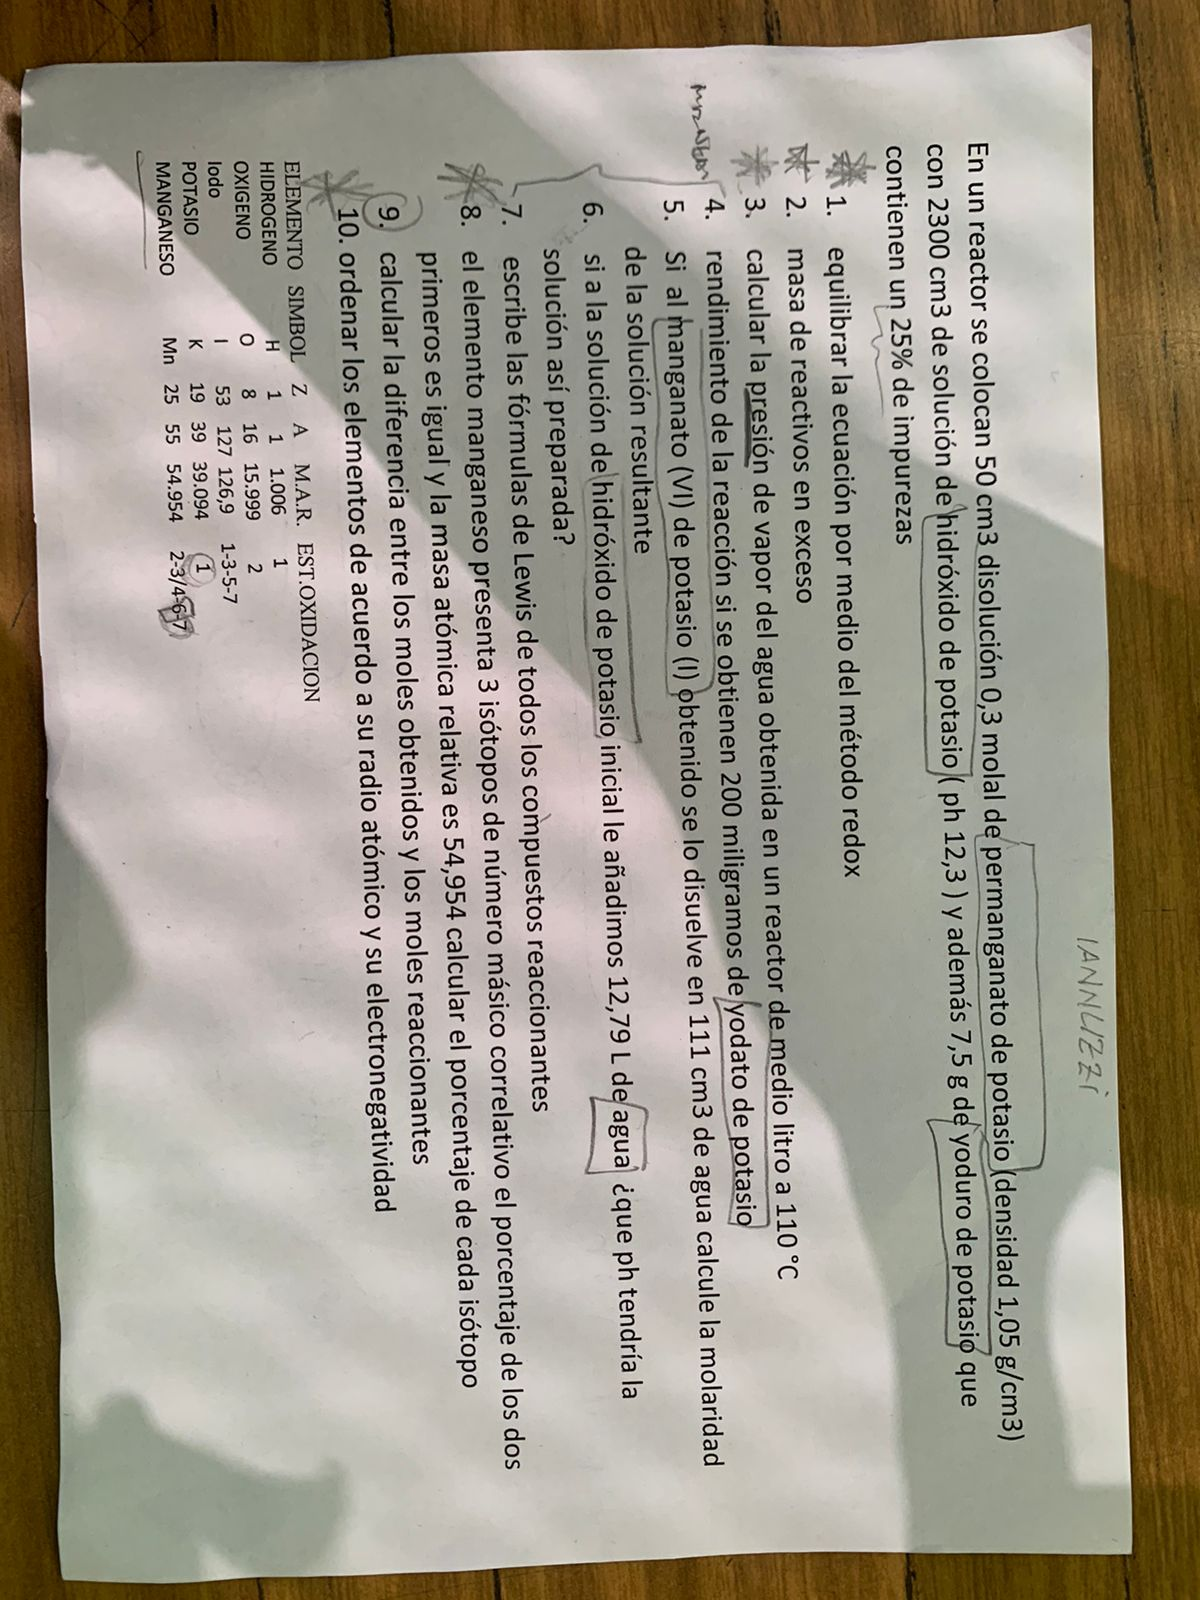
\includegraphics[width=0.7\linewidth, angle=90]{Images/molinos_examen1.jpg}
\end{figure}

\subsection*{Resolución}

\begin{enumerate}
\setlength\itemsep{2\baselineskip}

\item Balanceo por redox:
$$\ce{KMnO_4 + KOH + KI -> KIO_3 + K_2MnO_4}$$

Escribo los números de oxidación:
$$\ce{K^{+1}Mn^{+7}O_4^{-2} + K^{+1}O^{-2}H^{+1} + K^{+1}I^{-1} -> K^{+1}I^{+5}O_3^{-2} + K_2^{+1}Mn^{+6}O_4^{-2}}$$

Identifico cuál se oxida, cuál se reduce, al agente oxidante y al agente reductor:
\begin{table}[H]
    \centering
    \begin{tabular}{ll}
    Se oxida: & I \\
    Se reduce: & Mn \\
    Agente oxidante: & \ce{KMnO_4} \\
    Agente reductor: & \ce{KI}
    \end{tabular}
\end{table}

Identifico que es medio básico, planteo las semirreacciones, las balanceo e igualo los electrones:
\begin{multicols}{2}
    \underline{Semirreacción de oxidación:}
    $$\ce{I^- + 6OH^- ->
    IO_3^- + 3H_2O + 6e^-}$$
    
    \underline{Semirreacción de reducción:}
    $$\left( \ce{MnO_4^- + e^-  ->
    MnO_4^{2-}} \right) \cdot 6$$
\end{multicols}

Sumo las semirreacciones: 
$$\ce{
I^- + 6 OH^- + 6MnO_4 + \xcancel{6e^-} -> IO_3^- + 3H_2O + 6 MnO_4^{2-}\xcancel{6e^-}
}$$

Finalmente se ponen los coeficientes en la reacción original:
$$\fbox{\ce{6KMnO_4 + 6KOH + KI ->
KIO_3 + 6K_2MnO_4 + 3H_2O}}$$


\item Masa de reactivos en exceso:
$$\ce{6KMnO_4 + 6KOH + KI ->
KIO_3 + 6K_2MnO_4 + 3H_2O}$$

Calculo los moles de \ce{KMnO_4}:

\hfil$V_{\text{SC}}=50\text{cm}^3$
\hfil0,3m
\hfil$\delta = 1,05 \frac{\text{g}}{\text{cm}^3}$
\hfil $M = 158\frac{\text{g}}{\text{mol}}$

\hfil
Hay $2,37\text{g}\equiv 0,015 \text{mol}$ de $\ce{KMnO_4}$
\hfil

Calculo los moles de \ce{KOH}:

\hfil $V_{\text{SC}}=2,3 L$
\hfil pH = 12,3
\hfil 

\hfil
Hay $2,576\text{g} \equiv 0,046 \text{mol}$ de KOH
\hfil

Calculo los moles de \ce{KI}:

\hfil $m_i = 7,5g (\text{pureza}75\%)$
\hfil $M = 166\frac{\text{g}}{\text{mol}}$
\hfil

\hfil
Hay $5,625\text{g} \equiv 0,0339 \text{mol}$ de KI
\hfil

El limitante es \ce{KMnO_4}. Sobran 0,031 mol $\equiv$ 1,74g de KOH y 0,0314 mol $\equiv$ 5,21 g de KI.

Finalmente: 

\hfil
\fbox{masa de reactivos en exceso = 6,95 g}
\hfil


\item Presión del vapor del agua obtenida en un reactor de medio litro a 110ºC:
\begin{align*}
    P \cdot 0,5 \text{ l} &= 0,0075 \text{ mol} \cdot 0,082 \frac{\text{l}\cdot \text{atm}}{\text{mol} \cdot \text{K}} \cdot 383 \text{ K}\\
    P &= \dfrac{0,236 \text{ atm}}{0,5}\\
    \Aboxed{P &= 0,471\text{ atm}}
\end{align*}


\newpage
\item 0,2 g de \ce{KIO3} es $9,35\cdot 10^{-4}$ mol.

Con un rendimiento del \%100:
\rot{6}{1}{0,015}{2,5\cdot 10^{-3}}{mol de \ce{KMnO4}}{mol de \ce{KIO3}}

El rendimiento final es:

\hfil\fbox{
$\dfrac{9,35\cdot 10^{-4}}{2,5 \cdot 10^{-3}} \cdot 100\%
= 37,4\%$
}\hfil


\item Se obtienen $0,015\cdot 0,374 = 0,00561$ mol de \ce{K2MnO4}
\rot{0,00561}{0,111}{0,0505}{1}{mol}{l}
\hfil\fbox{
M = 0,0505
}
\hfil


\item 2,3 l de KOH, pH=12,3, le agrego 12,79 l de agua, calcular pH final.

\hfil $\text{pH}=12,4 \Rightarrow \text{pOH} = 1,7 \Rightarrow \left[\ce{OH^-}\right] = 10^{-1,7} = 0,02 $
\hfil
\rot{0,02}{1}
{0,046}{2,3}
{mol de \ce{OH^-}}{L}

Luego de diluir:
\rot{0,046}{15,09}
{3,05\cdot 10^{-3}}{1}
{mol de \ce{OH^-}}{L}

Finalmente:

\hfil \fbox{
$\text{pOH} = -\log\left( 3,05 \cdot 10^{-3} \right) = 2,52 \Rightarrow \text{pH} = 11,48$
}\hfil


\item xd

\item $A_1=53,\ A_2=54 y\ A_3=55.$
\begin{align*}
    53 \cdot p + 54 \cdot p + 55 \cdot (1 - 2p) &= 54,954\\    
    55 - 3p &= 54,954\\
    0,046 &= 3p\\
    p &= 0,0153
\end{align*}

Finalmente:

\hfil \fbox{
$p_1 = 1,53 \%,\ p_2 = 1,53 \%,\ p_3= 96,94 \%$
}\hfil


\item Sabiendo que reaccionan 0,015 mol de \ce{KMnO4}:

Moles obtenidos:

\hfil
0,015 mol \ce{K2MnO4} + 0,0075 mol de \ce{H2O} + 0,00375 mol de \ce{KIO3} = 0,02625 moles obtenidos
\hfil

Moles reaccionantes:

\hfil
0,015 mol \ce{KMnO4} + 0,015 mol de \ce{KOH} + 0,00375 mol de \ce{KI} = 0,03375 moles reaccionantes
\hfil


Finalmente:

\hfil \fbox{
$0,02625 - 0,03375 \text{ mol } = -0,0075\text{ mol}$
}\hfil


\item Radio atómico: H, O, K, Mn, I.
\hfil
Electronegatividad: K, Mn, H, I, O.
\hfil

\end{enumerate}


\end{document}

%%   http://detexify.kirelabs.org/classify.html
%%   https://oeis.org/wiki/List_of_LaTeX_mathematical_symbols

%%  Documento hecho por Ezequiel Mundani Vegega
